T\+O\+DO\+: add a part about graph created starting from c short circuits

Language based specification usually are translated into intermediate representations to efficiently manage and analyze the design specification. Panda as intermediate representation uses different types of graph. They can be divided into two main class\+:


\begin{DoxyItemize}
\item Representation at operation level\+: in these types of graphs every vertex corresponds to an operation and every edge corresponds to a precedence or a dependence (all graphs in this class are directed). There are also two nodes which doesn\textquotesingle{}t correspond to any real operation\+: E\+N\+T\+RY and E\+X\+IT. The first represents the specification begining, the second the specification ending. In all graphs there all vertices are directed connected to node E\+N\+T\+RY. The graphs which belongs to this class are\+:
\begin{DoxyItemize}
\item Control-\/\+Flow \hyperlink{structGraph}{Graph} (C\+FG)\+: it represents the control constructs of a description, like loops, branches, jumps, etc.
\item Control Dependence \hyperlink{structGraph}{Graph} (C\+DG)\+: it represents the control dependence of the description, i. e. by which operations the execution of every one is controlled
\item Data-\/\+Flow \hyperlink{structGraph}{Graph} (D\+FG)\+: since it is based of data dependency, it is the most parallel representation of the description. It Nevertheless it is not sufficient to fully represent control intensive representations.
\item Anti-\/dependencies (A\+DG) represents data dependences of type write after write and write after read
\item System Dependence \hyperlink{structGraph}{Graph} (S\+DG)\+: essentialy it\textquotesingle{}s equal to the merge of C\+DG and D\+FG
\item System Dependence and Antidependence \hyperlink{structGraph}{Graph} (S\+A\+DG)\+: System Dependence \hyperlink{structGraph}{Graph} plus Anti-\/\+Dependencies
\item Speculation \hyperlink{structGraph}{Graph}\+: System Dependence where some control dependences are eliminated in order to enable speculation in scheduling; there are also some edges added in order to reduce the possible speculation
\item Transitive reducted system dependence graph with feedback edges (R\+F\+S\+DG) (graph without feedback edges does not exist because it is not used)
\item Helping \hyperlink{structGraph}{Graph} (HG)\+: representation used by I\+LP scheduler
\end{DoxyItemize}
\item Representation at basic block level\+: in these types of graphs every vertex corresponds to a set of control equivalent operations (basic block)\+:
\begin{DoxyItemize}
\item Basic Block Control-\/\+Flow \hyperlink{structGraph}{Graph} (BB)\+: it represents the control constructs of a description at basic block level
\item Dominator Tree (DT)\+: dominator tree built on Basic Block Control-\/\+Flow \hyperlink{structGraph}{Graph}
\item Post-\/\+Dominator Tree (P\+DT)\+: post-\/dominator tree built on Basic Block Control-\/\+Flow \hyperlink{structGraph}{Graph}
\end{DoxyItemize}
\end{DoxyItemize}

For many of these types of graphs there are two different version\+: the first hasn\textquotesingle{}t feedback edges, the second does. An edge is of feedback type if it closes a cycle in some path starting from E\+N\+T\+RY.

In following subsection all types will be more accurately described and it will be given the correspondent graph of the following example\+: \begin{DoxyVerb} 1  a = 1;
 2  b = 2;
 3  c = 3;
 4  d = 0;
 5  a = a + b;
 6  e = a == b;
 7  if (e)
    {
 8    c = a + b;
      do
      {
 9      h = c + d;
10      c = c + 1;
11      d = d + 1;
12      g = c + d;
13      f = d !=c ;
      }
14    while(f);
    }
15  c = c + d;
16  c = c + 1;
\end{DoxyVerb}


The control flow graph represents the sequencing of the operations as described in the language specification. The C\+FG is a directed graph whose vertexes are represented by set V = \{ $v_i$ ; i = 1, 2, ... , $no_p$ \}. The set of edges is E = \{( $v_i$ , $v_j$ ); i , j = 1, 2, ... , $no_p$ \}. It takes into account all constructs that cause a re-\/direction of the computational flow, such as branch statements, loop statements, jump statements, etc. The advantages of this representation is that it is quite simple to extract from the system specification even if it does not express the potential parallelism of the operations.

On the other side one of the main disadvantages is that C\+FG generation for multi-\/process systems specifications does not appear to be simple, since a C\+FG has to manage at the same time all the flows of control of all the processes that compose the system. Thus the C\+FG model results intrinsically suitable just for single-\/process descriptions.

Some of the algorithms and tools which work on graph in PandA assume that the only type of cycle construct present in specification is the repeat-\/until. So if in specification some while-\/construct is present, it will be transformed into a \char`\"{}if repeat until\char`\"{} structure.

An example of C\+FG is\+: 
\begin{DoxyImageNoCaption}
  \mbox{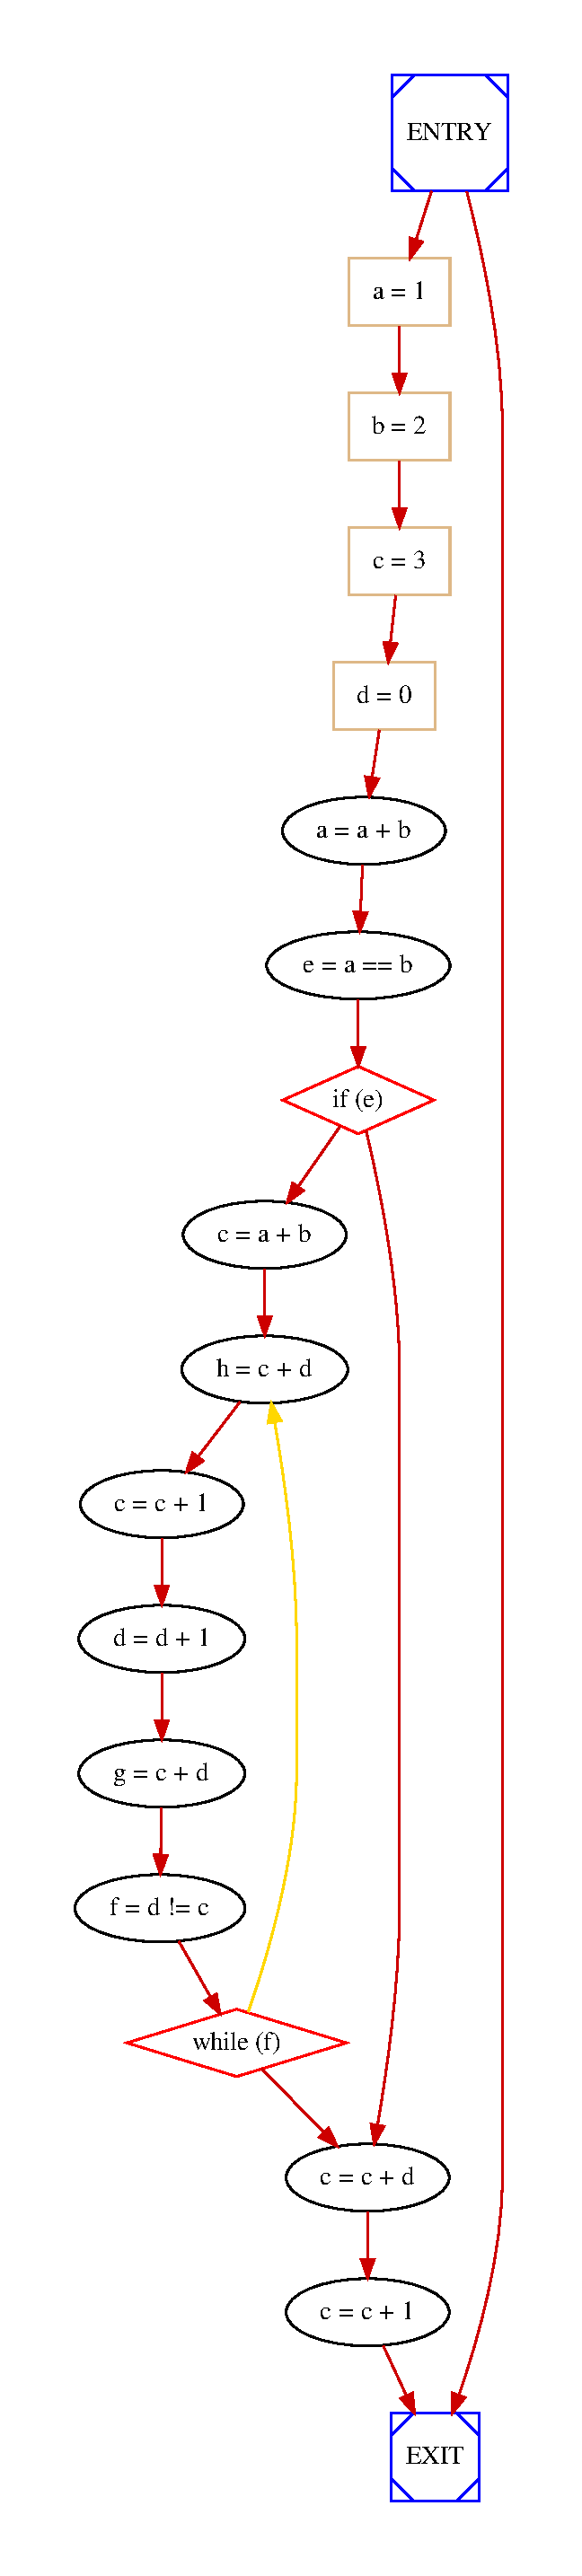
\includegraphics[width=\textwidth,height=\textheight/2,keepaspectratio=true]{dot_inline_dotgraph_1}}
\end{DoxyImageNoCaption}
 As you can see diamond nodes represent selection operations (e.\+g. T\+Y\+P\+E\+\_\+\+IF nodes), box nodes represent assignmente operations and square boxes represent special operations (E\+N\+T\+RY, E\+X\+IT and functions call which are not present in the given simple example)

The Control-\/\+Dependence graph represents control dependencies within operations, e. g. from which operation the excution of a single operation is controlled. We say that a node y is control-\/dependent on x if in C\+FG (for the moment we do not consider control flow feedback edges) from x we can branch to u or v; from u there is a path to exit that avoids y, and from v every path to exit hists y\+: 
\begin{DoxyImageNoCaption}
  \mbox{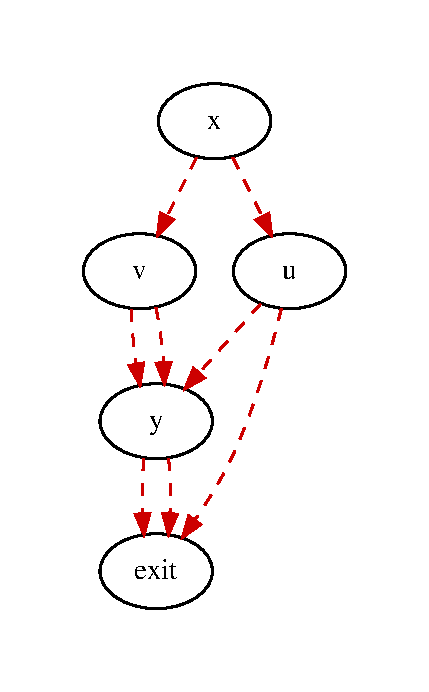
\includegraphics[width=\textwidth,height=\textheight/2,keepaspectratio=true]{dot_inline_dotgraph_2}}
\end{DoxyImageNoCaption}
 The C\+DG used in PandA has not only an edge between every pair (x,y) where y is control-\/dependent on x, but also from every node belonging to a cycle to ifs at the end of that cycle. In this mode we forced the check of the condition of the loop to be executed after all the operation of the cycles.

Moreover the in case of loop we also add some control dependence feedback edges\+: there is a control dependence feedback edge from every if which ends the loop to all operation which starts a new flow in the loop body, e. g. each operation which has control or data dependence only from operations external to loop body. An example of C\+DG is\+: 
\begin{DoxyImageNoCaption}
  \mbox{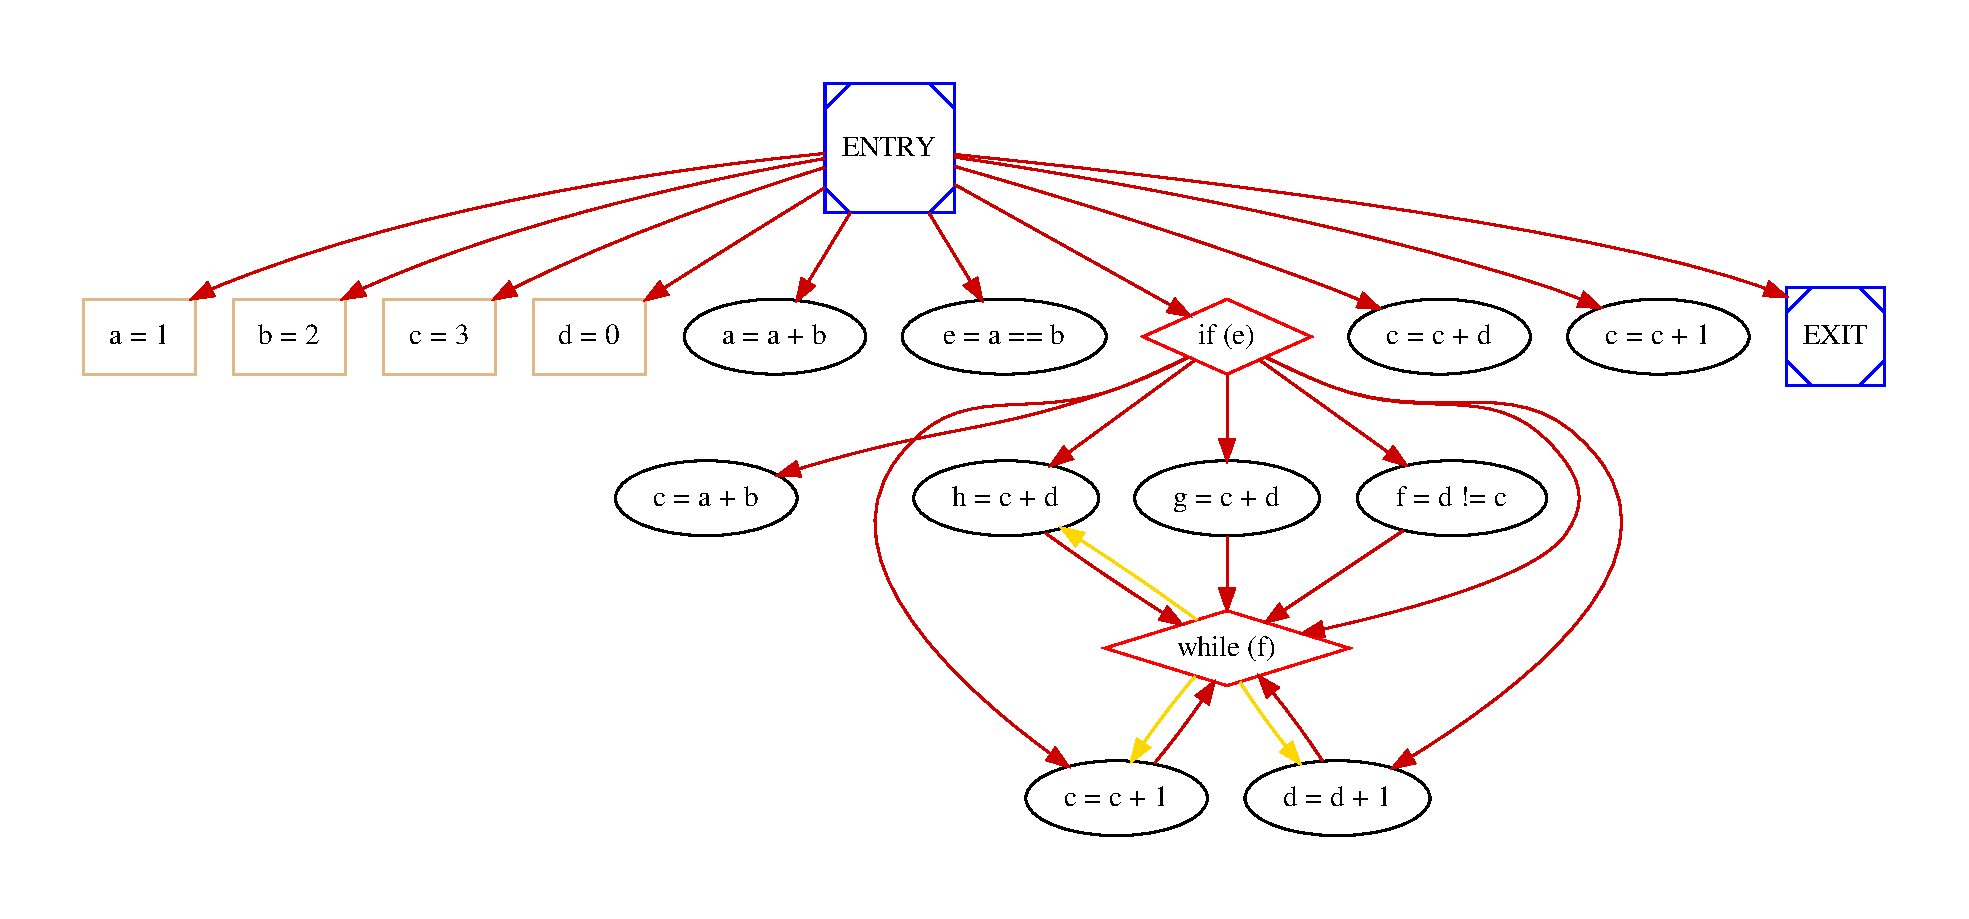
\includegraphics[width=\textwidth,height=\textheight/2,keepaspectratio=true]{dot_inline_dotgraph_3}}
\end{DoxyImageNoCaption}


The data flow graph represents operations and data dependencies only of type read after write. A D\+FG is a directed graph whose vertexes are represented by the set V = \{ $v_i$ ; i = 1, 2, ... , $no_p$ \}, where $no_p$ is the number of operations. The set of edges E = \{( $v_i$ , $v_j$ ); i , j = 1, 2, ... , $no_p$ \} represents the data transfer from an operation to another one. The D\+FG model implicitly assumes the existence of variables, that store the information required and generated by the operations. Each variable has a lifetime and the model assumes that the values of the variables are preserved during their lifetime. The lifetime of a variable is the interval from the birth and the death of the variable. The birth is the time at which the value is generated as output of an operation, the death is the latest time at which the variable is used as input to an operation. An Example of D\+FG is\+: 
\begin{DoxyImageNoCaption}
  \mbox{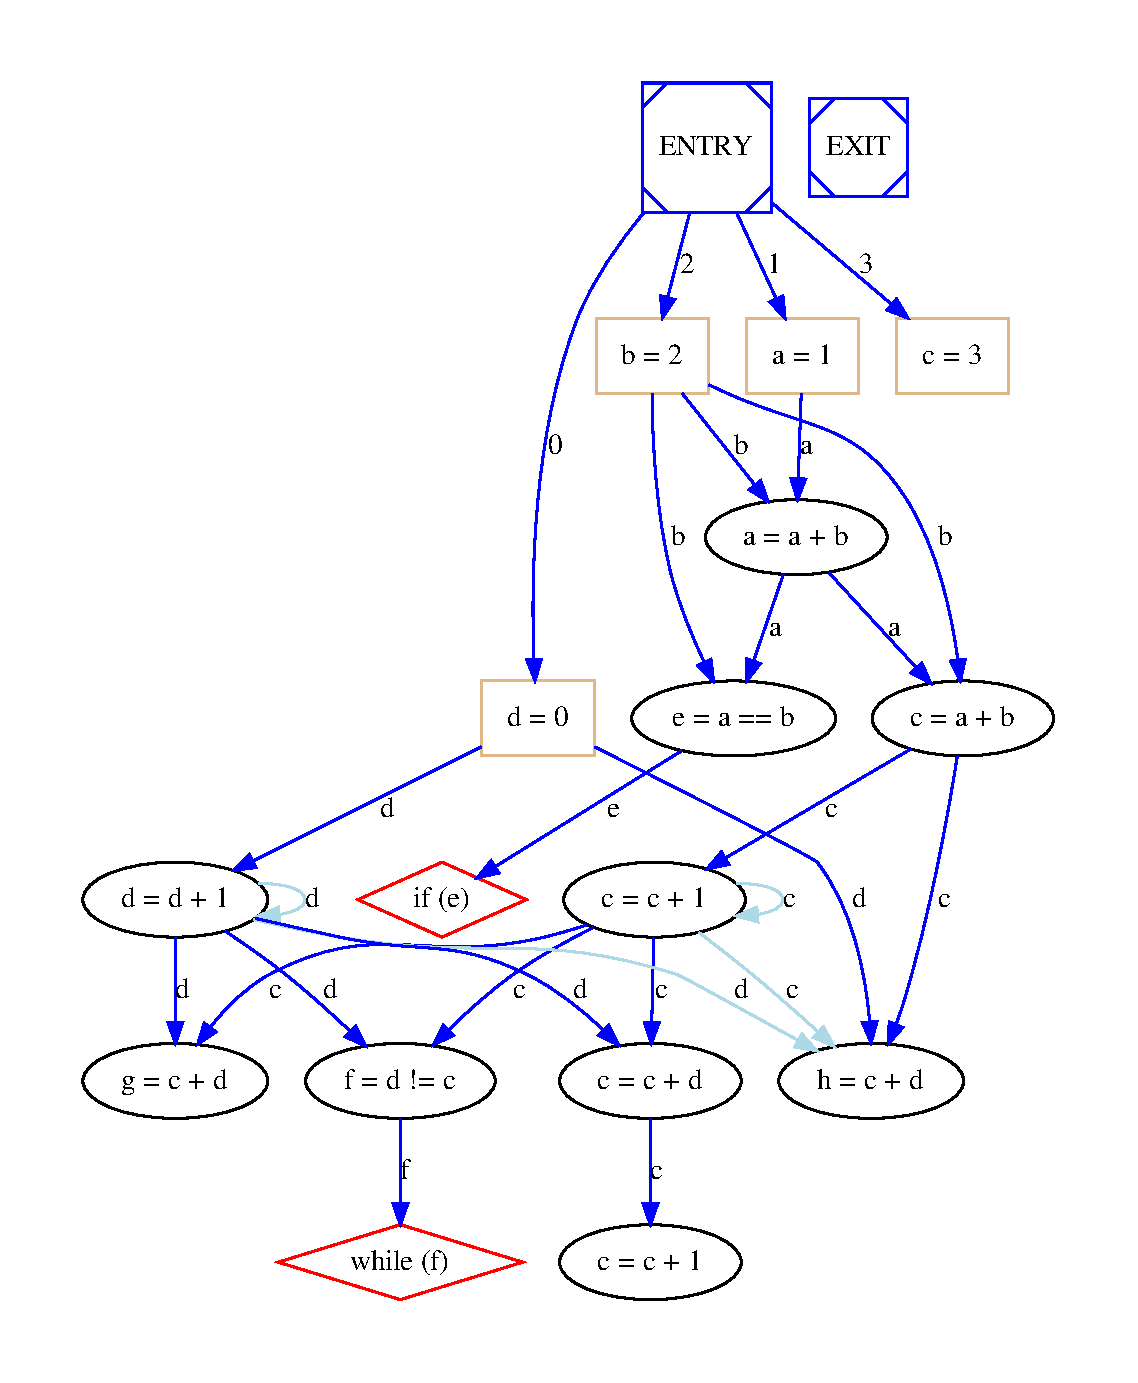
\includegraphics[width=\textwidth,height=\textheight/2,keepaspectratio=true]{dot_inline_dotgraph_4}}
\end{DoxyImageNoCaption}


The Anti-\/dependence-\/graph represents operations and data dependencies of type write after write and write after read. These dependencies assure that variable reading and writing follows strict consistency model. Note that if in the original specification there are two writes (definitions) of the same variable and there isn\textquotesingle{}t a use of the first definition, in the PandA representation the first operation does not write the variable, so in this case the Anti-\/dependence will not be added. The problem of variable consistency model and then the problem of Anti-\/dependencies are present only in case of not using S\+SA (Static Single Assingment) form\+: if we use it there are no more anti-\/dependencies. 
\begin{DoxyImageNoCaption}
  \mbox{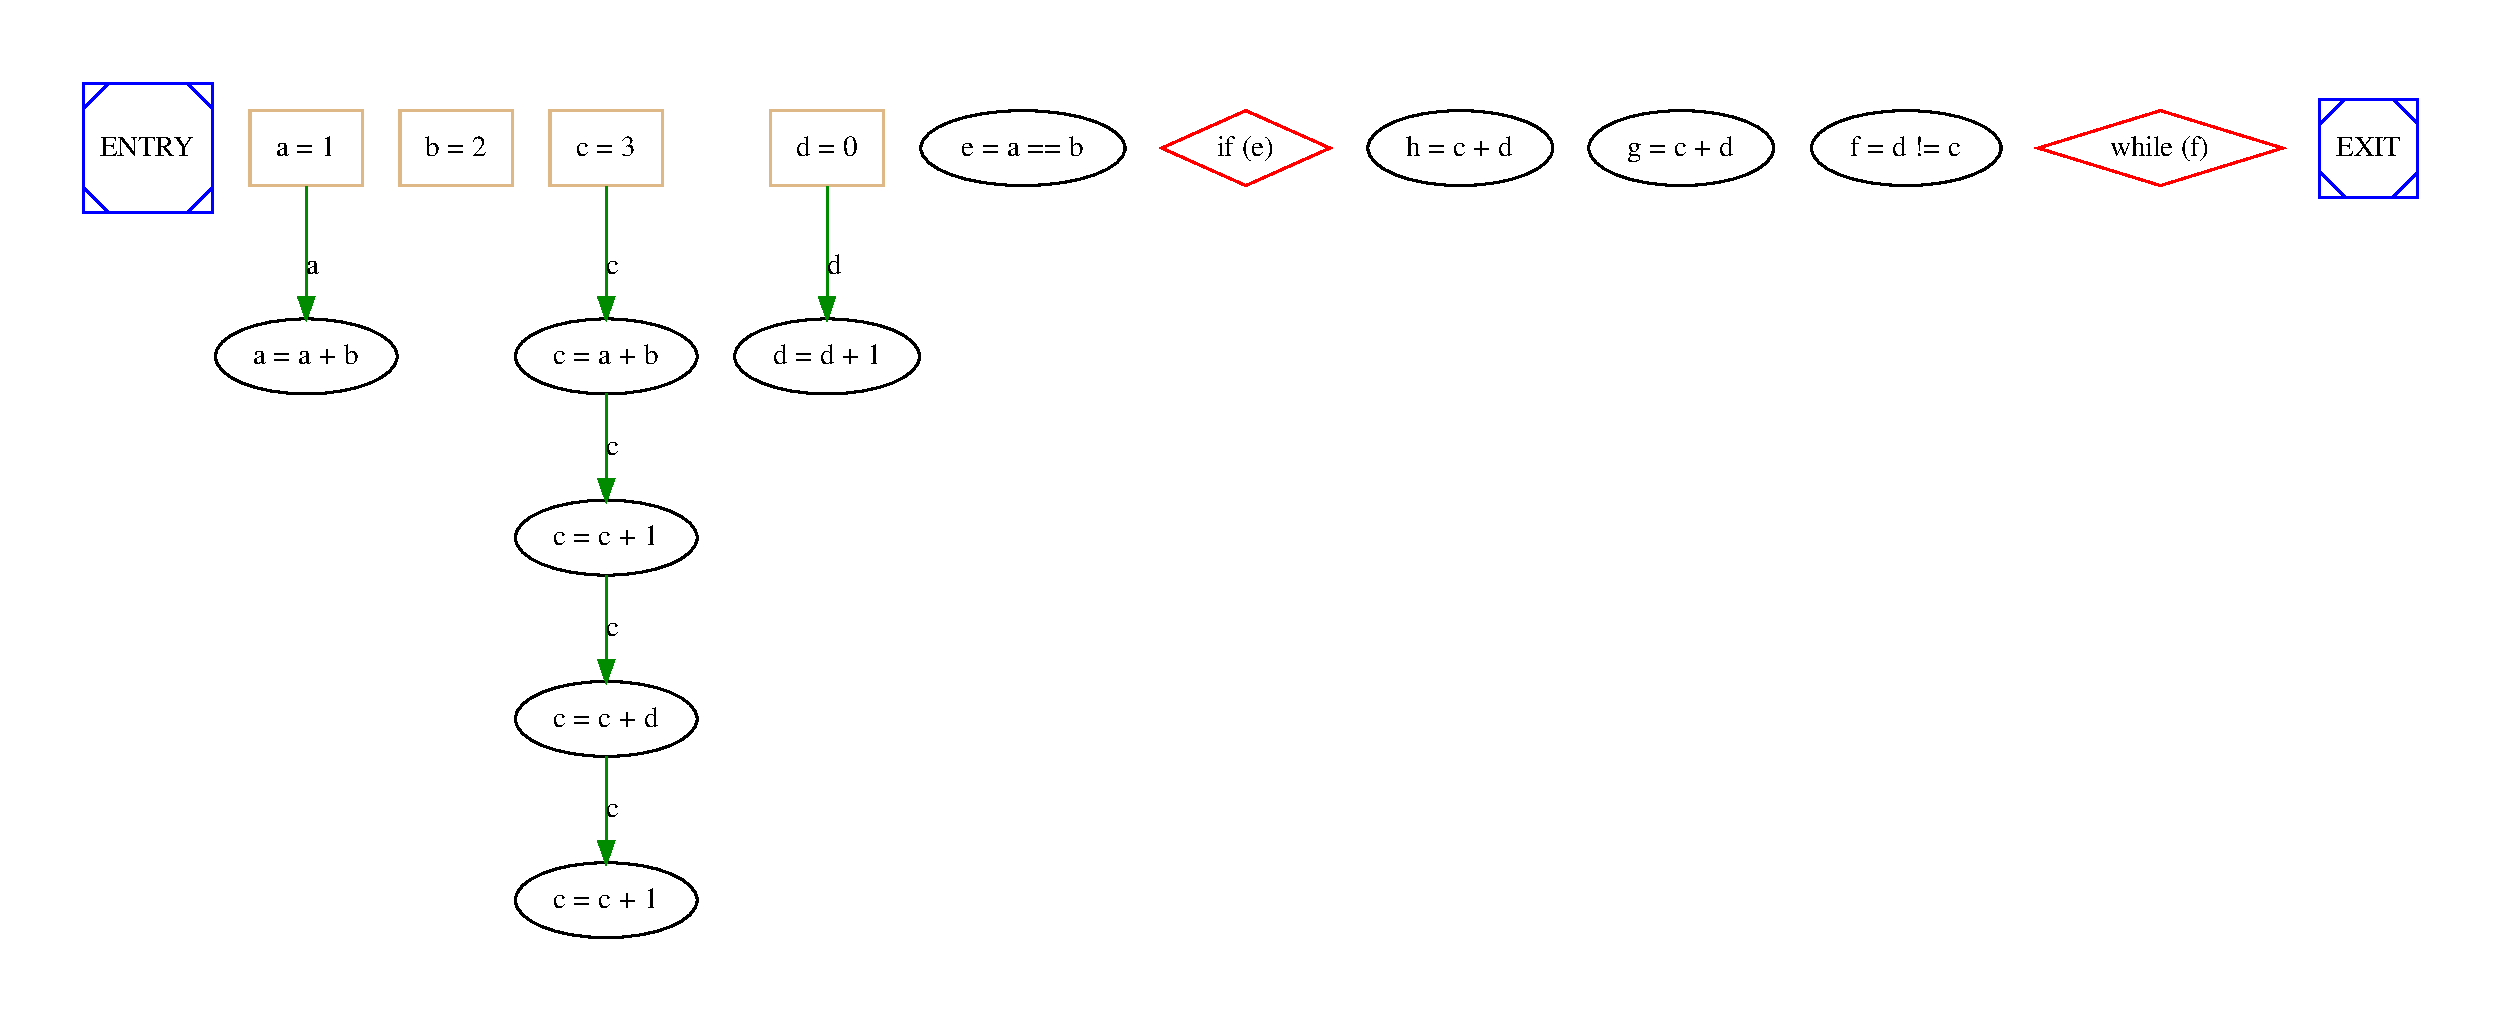
\includegraphics[width=\textwidth,height=\textheight/2,keepaspectratio=true]{dot_inline_dotgraph_5}}
\end{DoxyImageNoCaption}


The System dependence graph is the fusion of two graphs\+: Control-\/dependence graph and Data-\/flow graph. It\textquotesingle{}s useful because it represents both data and control dependence in an unique graph, but it does not contain futher precedences which are not real like control flow graph ones. It doesn\textquotesingle{}t no represent Anti-\/dependencies so it can be used by scheduling algorithms only if we are using S\+SA form. An example of S\+DG is\+: 
\begin{DoxyImageNoCaption}
  \mbox{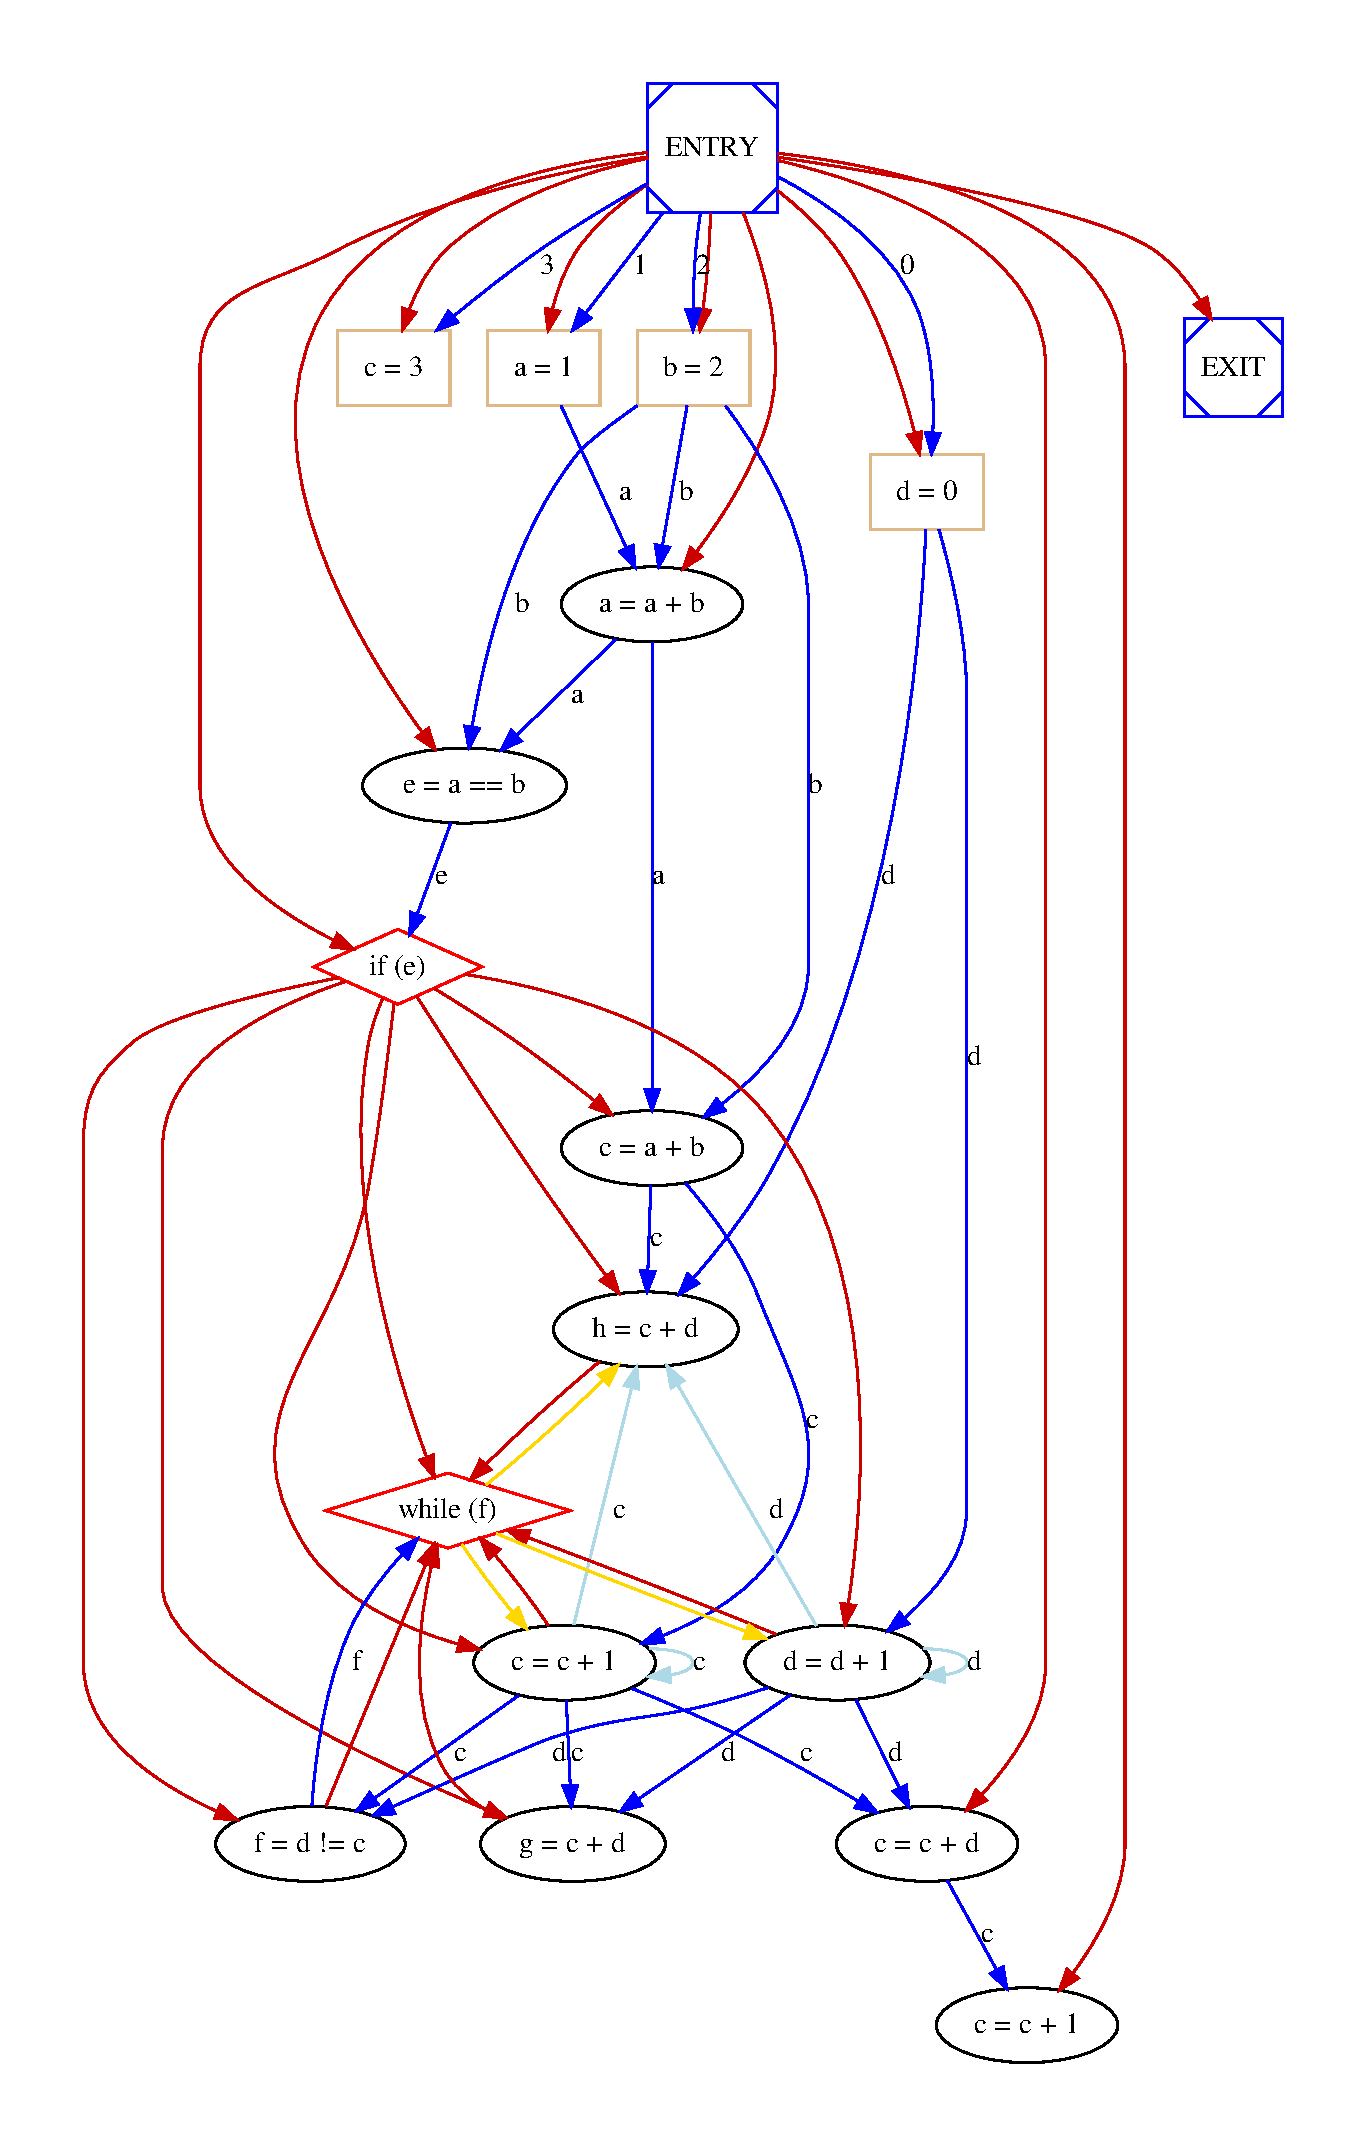
\includegraphics[width=\textwidth,height=\textheight/2,keepaspectratio=true]{dot_inline_dotgraph_6}}
\end{DoxyImageNoCaption}


The System dependence and anti-\/dependence graph is the fusion of three different graph\+: control dependence graph, data flow graph and Anti-\/dependence graph. For this reason it reperesents all type of dependence and precedence between operations and it can be used by scheduling alghorithm in order to compute scheduling. An example of S\+A\+DG is\+: 
\begin{DoxyImageNoCaption}
  \mbox{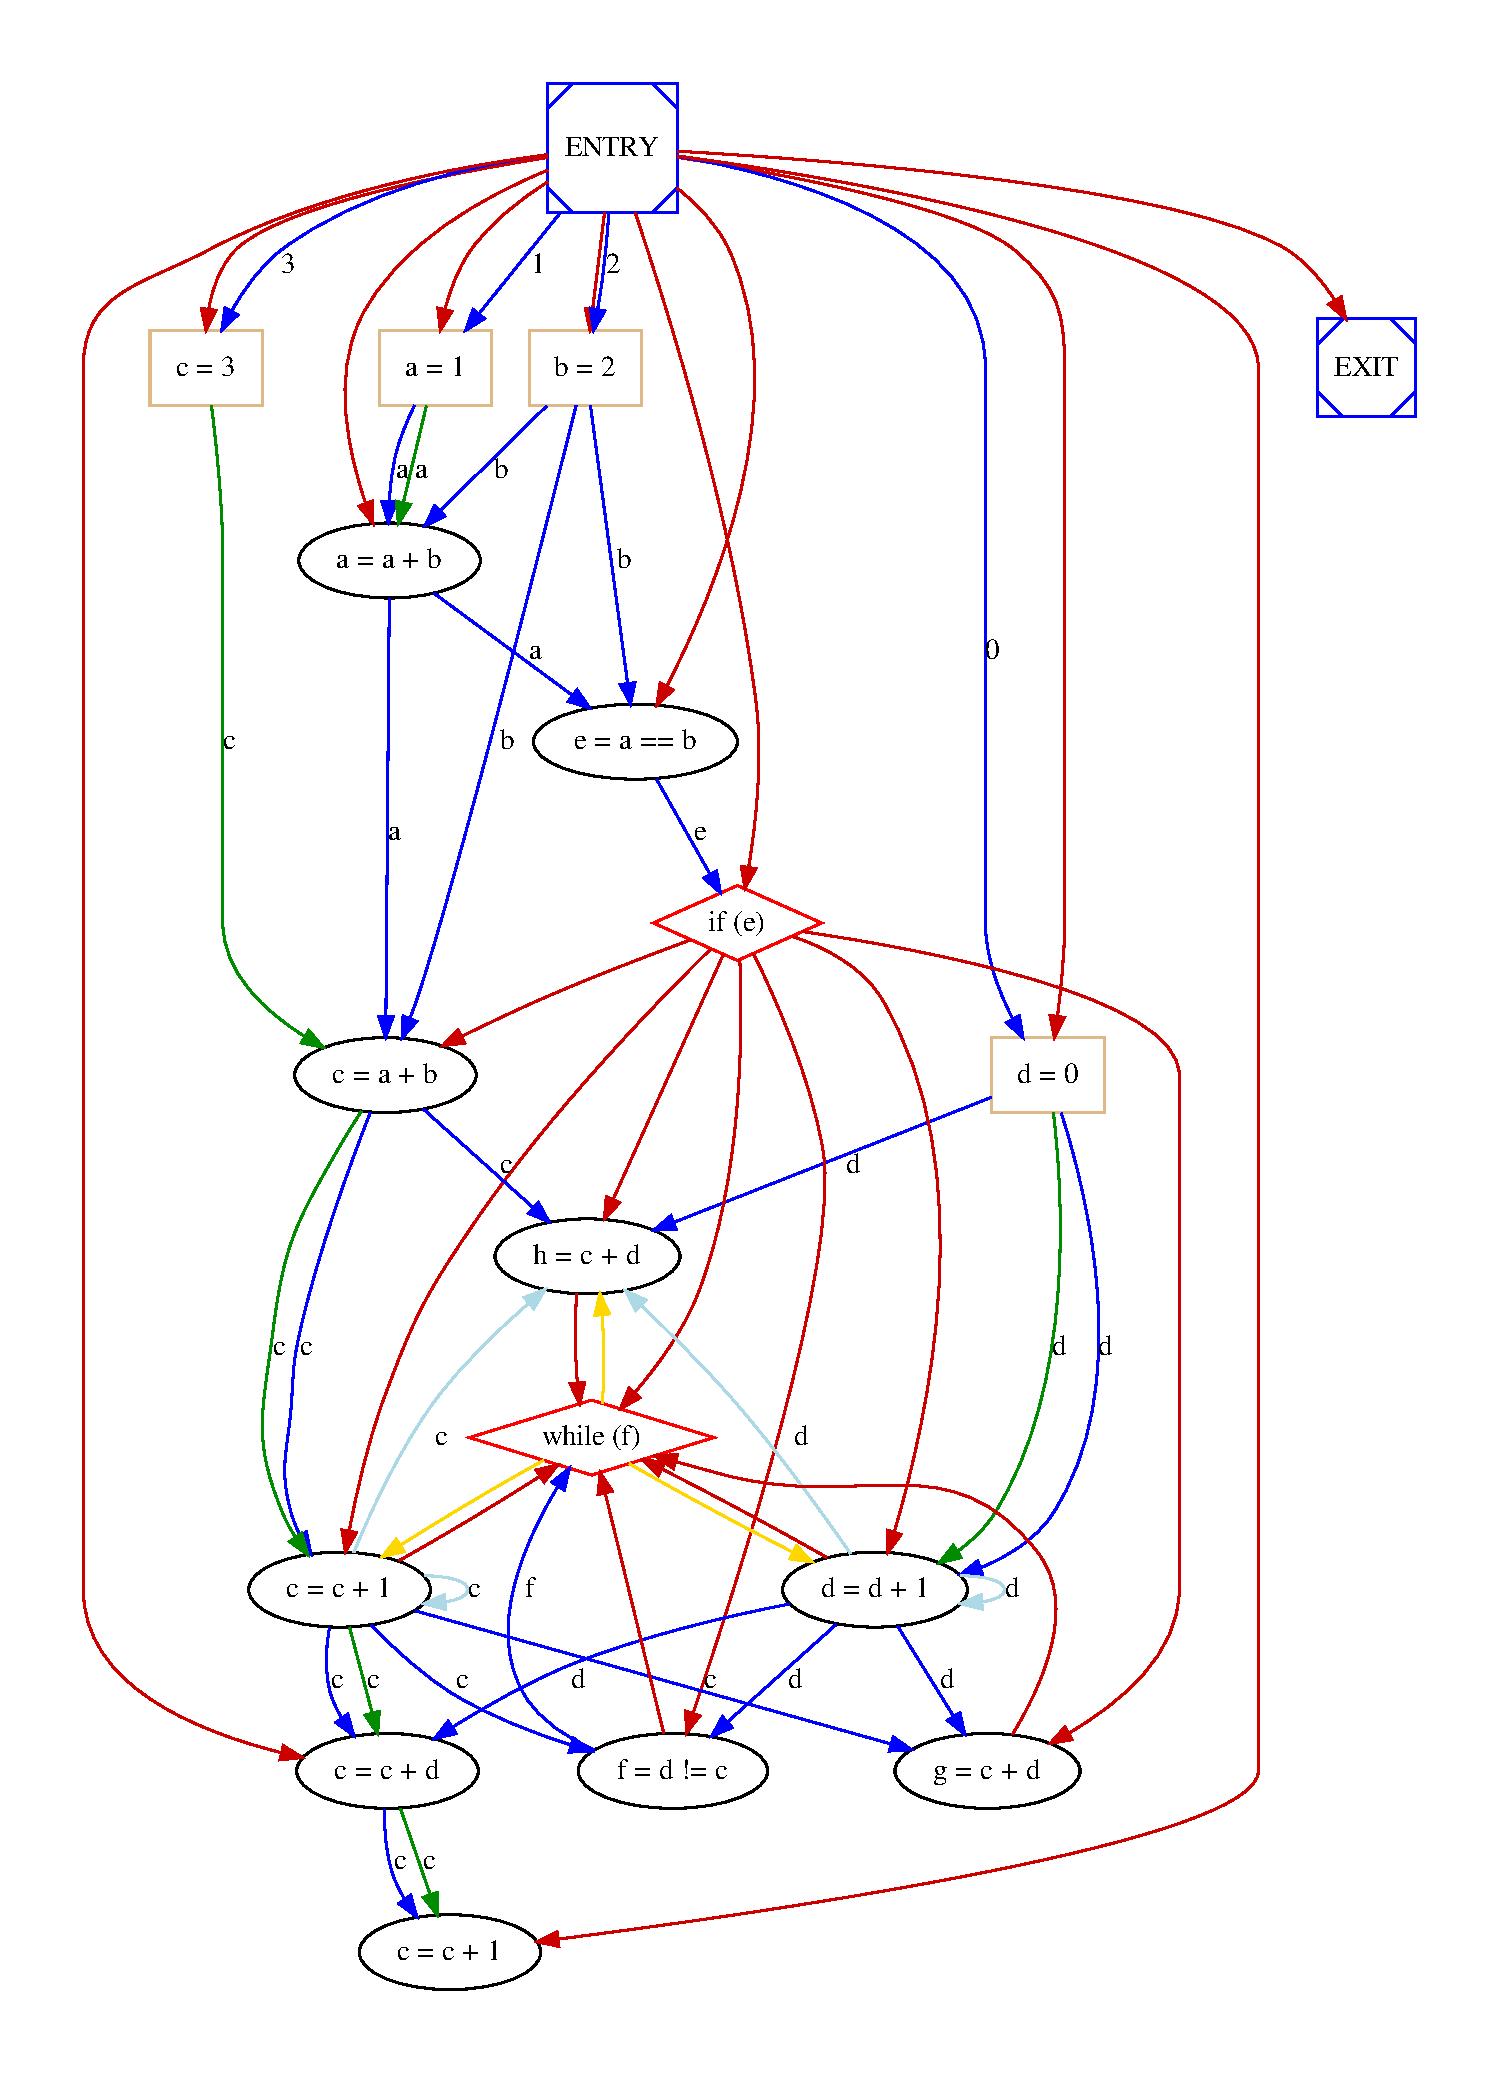
\includegraphics[width=\textwidth,height=\textheight/2,keepaspectratio=true]{dot_inline_dotgraph_7}}
\end{DoxyImageNoCaption}


Speculation graph is a modified version of S\+A\+DG where some control constraints are relaxed in order to permit control speculation in scheduling. This type of speculation consists in executing operations controlled by a controll construct like an if before that if condition and so the target of the control flow execution is computed. Doing this it is possible executing the specification in less time but it is also possible that more functional unit and a more complex controller is required in order to permit this techinique. In order to limitate the depth of speculation, it\textquotesingle{}s possible only to anticipate the execution of operations which directly dependes by a control construct but it is not possible to anticipate the execution of operation which depends inderectly by a chain control dependence plus other type of dependence (data or anti-\/dependence). An example of SG is\+: 
\begin{DoxyImageNoCaption}
  \mbox{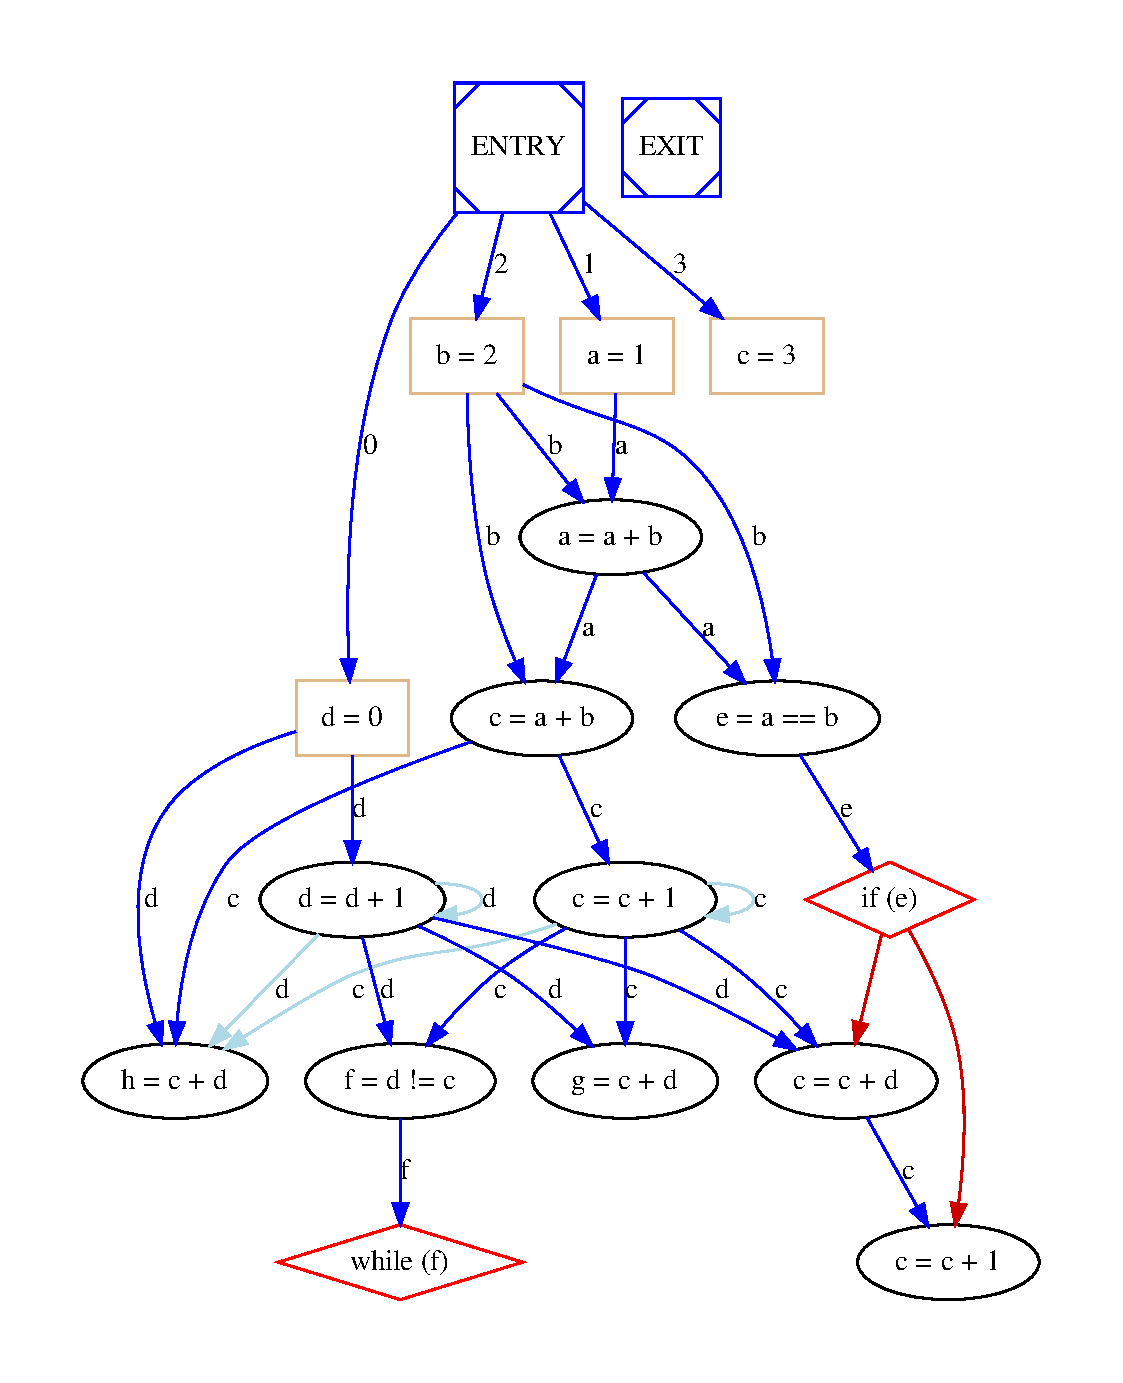
\includegraphics[width=\textwidth,height=\textheight/2,keepaspectratio=true]{dot_inline_dotgraph_8}}
\end{DoxyImageNoCaption}


A Basic Block is a sequence of operations that is always entered at the beginning and exited at the end, that is\+: -\/the first statement is a Label, e. g. a possible target of a jump; -\/the last statement is a conditional jump, e. g. a control construct; -\/there are no other labels or jumps. Basic blocks are usually the basic unit to which compiler optimizations are applied in compiler theory, because if during the execution the first operation of basic block is executed, all operations belonging to the same basic block will be executed.

Instructions which begin a new basic block include\+:
\begin{DoxyItemize}
\item Procedure entry points
\item Targets of jumps or branches
\item \char`\"{}\+Fall-\/through\char`\"{} instructions following some conditional branches
\end{DoxyItemize}

Instructions that end a basic block include\+:
\begin{DoxyItemize}
\item Unconditional and conditional branches, both direct and indirect.
\item Returns to a calling procedure.
\item Function calls can be at the end of a basic block if they may not return, such as functions which throw exceptions.
\end{DoxyItemize}

The Control flow graph of Basic Block is like previously described Control flow graph but the vertices instead of single operation are basic blocks. So in the version with feedback edges of this particular type of graphs it is not possible that a vertex has only one edge ingoing and a vertex has only one edge outgoing. The blocks to which control may transfer after reaching the end of a block are called that block\textquotesingle{}s successors, while the blocks from which control may have come when entering a block are called that block\textquotesingle{}s predecessors.

The algorithm for generating basic blocks from a listing of code is simple\+: you scan over the code, marking block boundaries, which are instructions which may either begin or end a block because they either transfer control or accept control from another point. Then, the listing is simply \char`\"{}cut\char`\"{} at each of these points, and basic blocks remain. Note that this method does not always generate maximal basic blocks, by the formal definition, but they are usually sufficient.

An example of BB Control Flow \hyperlink{structGraph}{Graph} is\+: 
\begin{DoxyImageNoCaption}
  \mbox{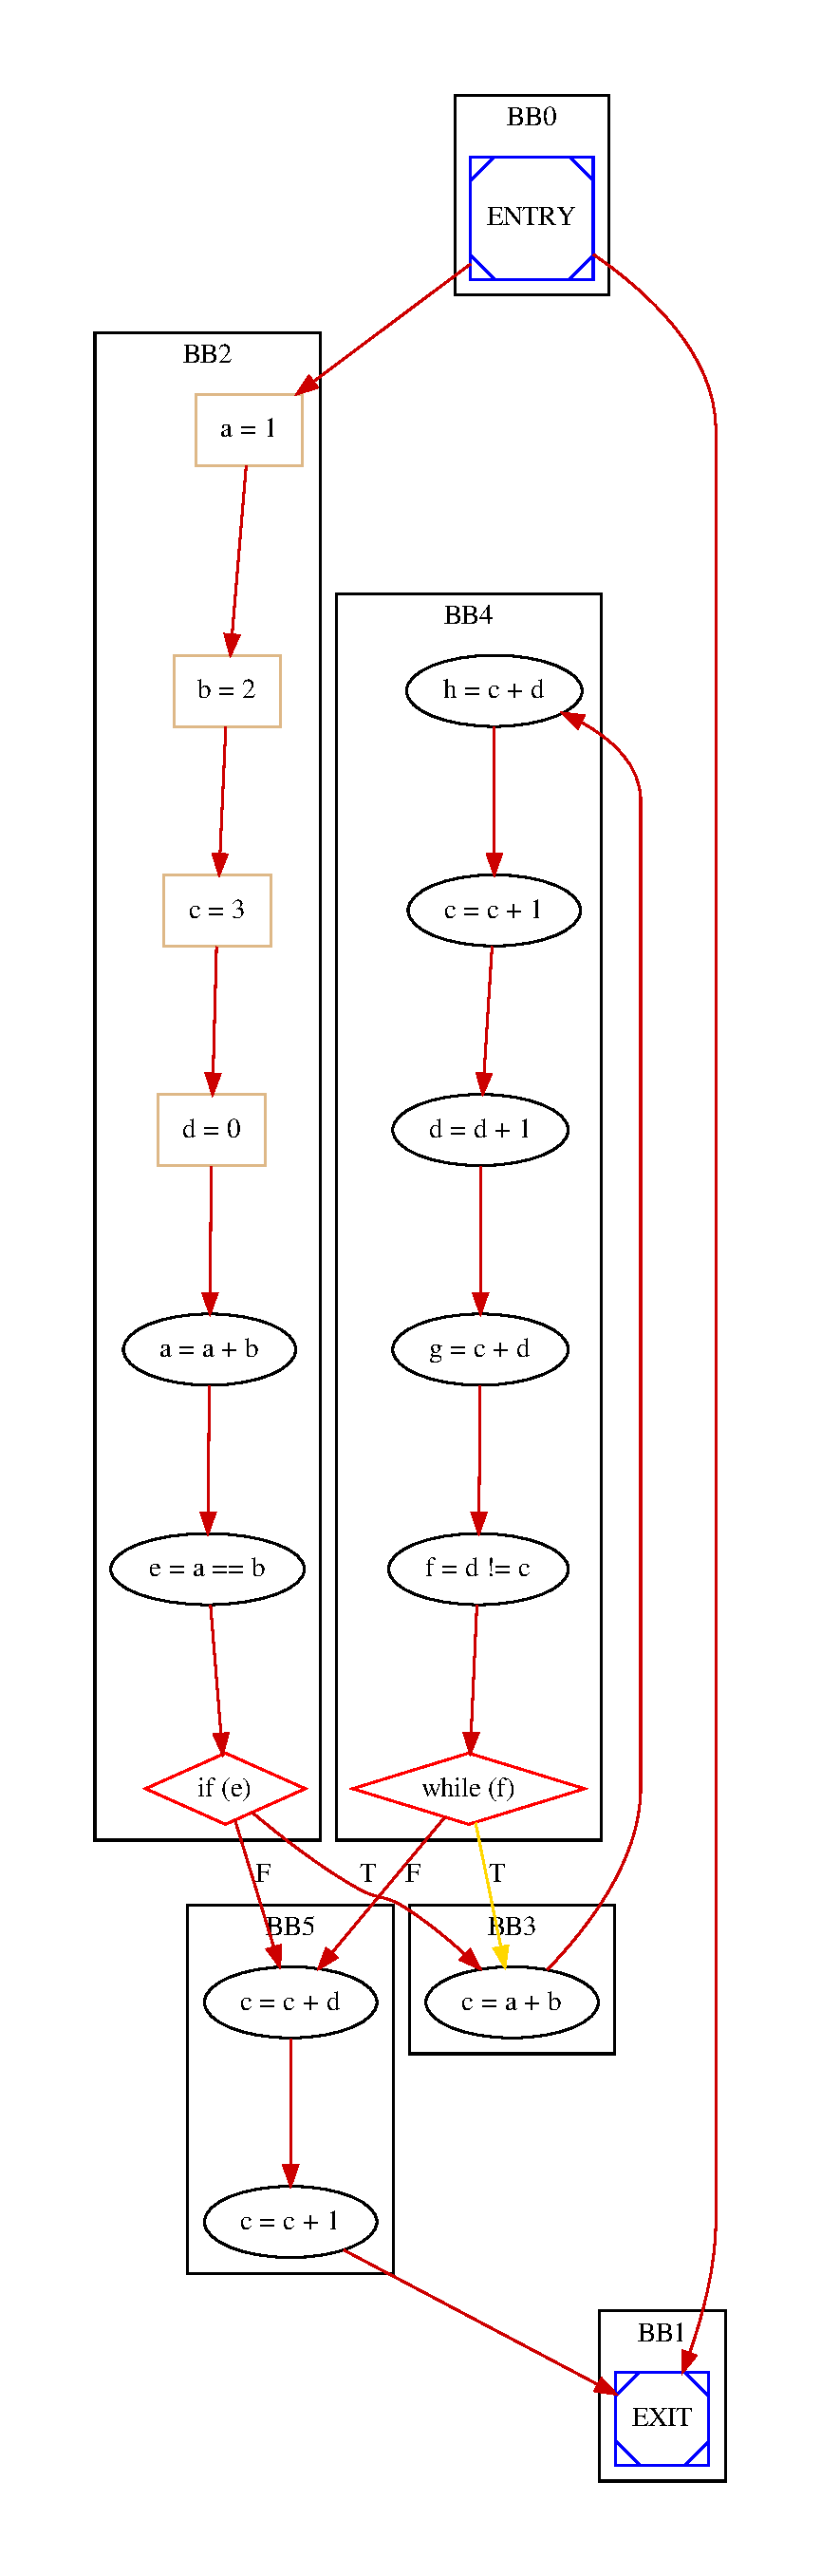
\includegraphics[width=\textwidth,height=\textheight/2,keepaspectratio=true]{dot_inline_dotgraph_9}}
\end{DoxyImageNoCaption}


In computer science, in compilers, a dominator is an object which is always executed before another object, where the object is typically either a statement or a basic block. By definition an object dominates itself as well. A block M dominates a block N if every path from the entry that reaches block N has to pass through block M. The entry block dominates all blocks. Note that an object may have many dominators. Sometimes more useful is the concept of an immediate dominator, which is the unique object that dominates an object, while not dominating any other dominator of the object. A block M immediately dominates a block N if M dominates N, and there is no intervening block P such that M dominates P and P dominates N . In other words, M is the last dominator on any path from entry to N . Each block has a unique immediate dominator, if it has any at all. In the Basic Block Control flow graph used in Panda every blocks but E\+N\+T\+RY has an immediate dominator.

The dominator tree is an ancillary data structure where each object\textquotesingle{}s parent is its immediate dominator. There is an arc from block M to block N if M is an immediate dominator of N. This graph is a tree, since each block has a unique immediate dominator. This tree is rooted at the entry block.

The dominators tree can be performed by using the Cooper algorithm \mbox{[}Keith D. Cooper, Timothy J. Harvey, Ken Kennedy, A Simple, Fast Dominance Algorithm, Software Practice and Experience, 2001.\mbox{]}, which is basically an iterative algorithm adopting some refinements in the data structures used. At a later stage it could be substituted with a more efficient one, like the algorithm of Lengauer and Tarjan.

An example of dominator tree built from the Basic Block C\+FG is\+: 
\begin{DoxyImageNoCaption}
  \mbox{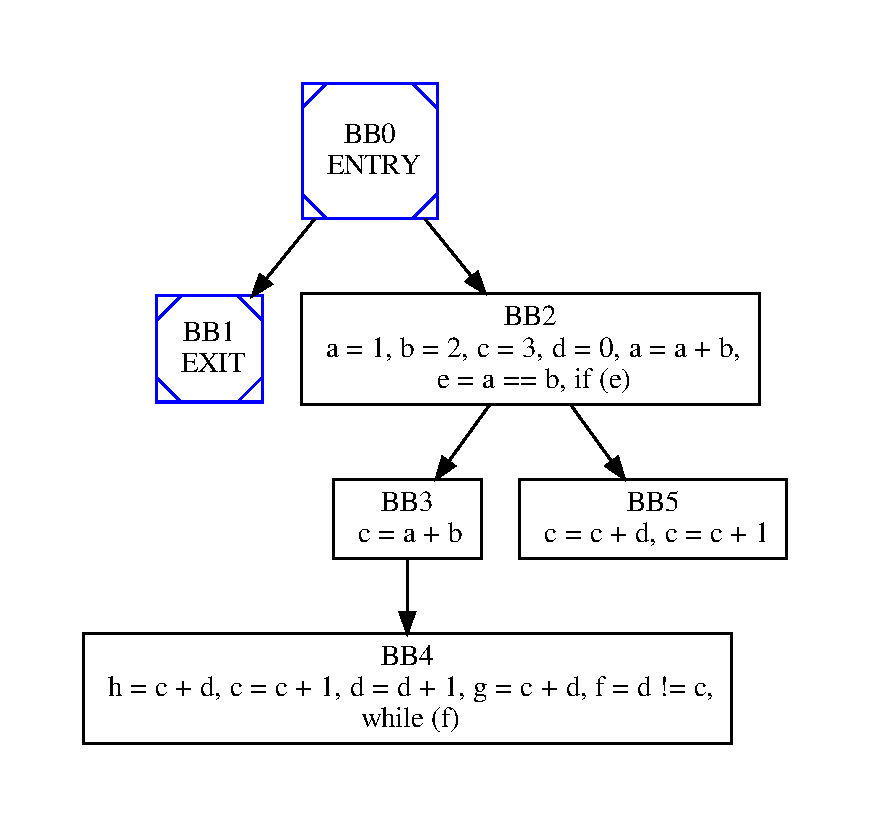
\includegraphics[width=\textwidth,height=\textheight/2,keepaspectratio=true]{dot_inline_dotgraph_10}}
\end{DoxyImageNoCaption}
 

The relationship of post-\/dominance is the dual of dominance relation\+: we say that y postdominates v when y is on every path fro v to E\+X\+IT. Following the dualism with dominance relationship it is possible to define the immediate post-\/dominance relationship and then to build the Post Dominator tree.

An example of Post-\/dominator tree built from Basic Block C\+FG is\+: 
\begin{DoxyImageNoCaption}
  \mbox{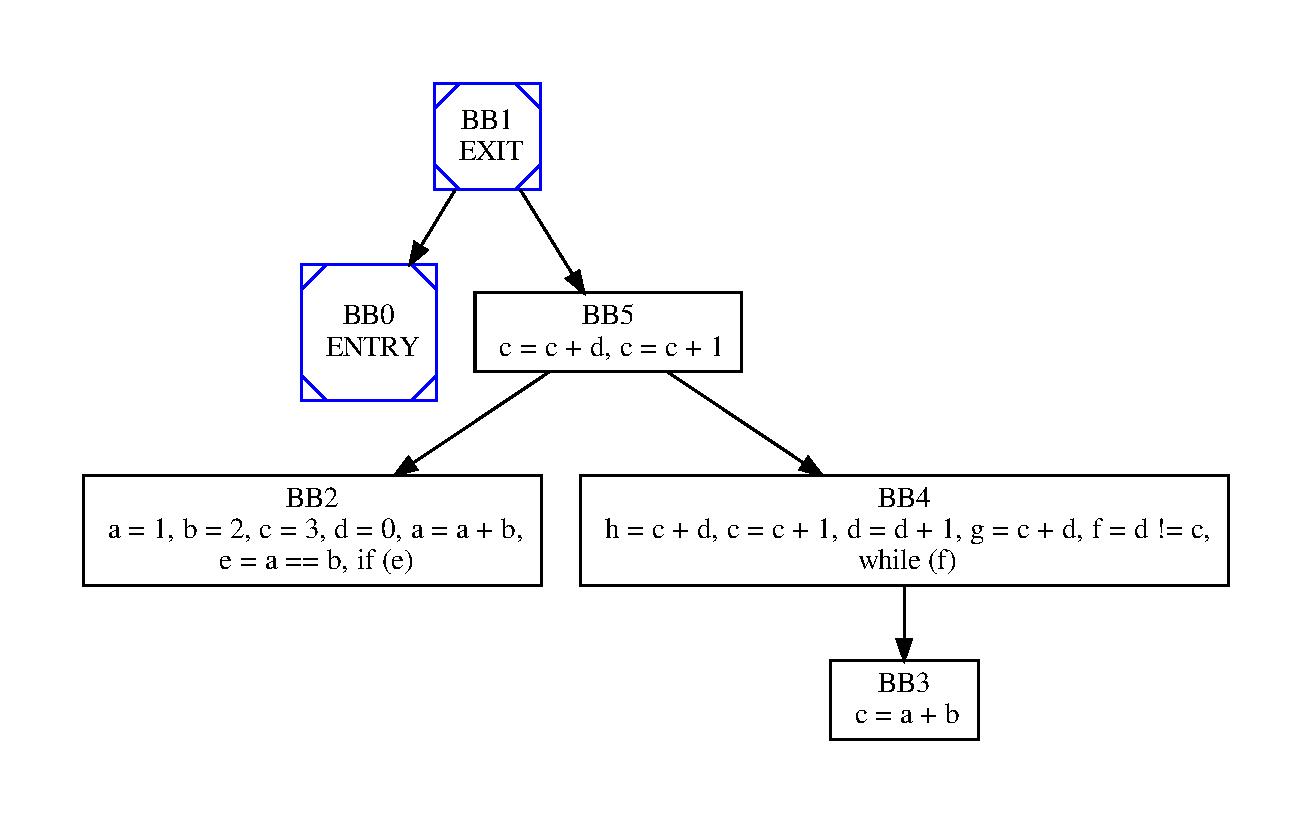
\includegraphics[width=\textwidth,height=\textheight/2,keepaspectratio=true]{dot_inline_dotgraph_11}}
\end{DoxyImageNoCaption}
 